\documentclass[]{article}

% Used packages
\usepackage{multicol} % allows to use multiple column alignment
\usepackage{graphicx} % allows to use graphics
\usepackage{caption} %allows more extensive caption formating

%opening
\title{Extracting objective facts \\ from subjective and noisy sources}
\author{Kirill Tumanov \& Panagiotis Chatzichristodoulou}

\begin{document}

\maketitle

\begin{abstract}
In a world where media coverage is big and one can easily be overflooded information, the need for automatic fact extraction is increasing by the day. News agencies over the world can present the same information under a different perspective, making it difficult for the reader to distinguish facts from opinions. The main goal of this work was to implement a framework that receives data from differently aligned sources and output the subjective facts that are hidden within the data. As a subject topic the highly controversial crisis in Ucraine was chosen, since it created strong opinions and due to that facts where masked behind subjective opinions.
\end{abstract}

%
\section{Introduction}
%
Modern news agencies discuss the ongoing events with a great deal of subjectivity and dispute. This may be related to the general complexity of the causal relations in each situation nowadays, but also to the desire to put the events in a different light so that their story sells best. Whichever the reason is it is becoming more and more demanding for the reader to grasp what actually is going on. Especially when it comes to the analysis of the several information sources.

Today it is very popular to discover and evaluate polarity of the opinions on the web by emotional and sentiment mining. This analysis is useful specifically for uncovering of the (mostly author's) attitude towards the situation. However, it does not provide any insight in what exactly was criticized or admired. In other words, it does not provide the context for the overall result, it just presents the attitude.

When a more pragmatic and detailed analysis is needed, fact extraction comes into play. An underlying basis of the present work is the belief that the proper information presentation is free of the emotional flavor, and that each story is comprised of a set of interrelated facts and events. When it comes to understanding the situation, only facts matter.

An example of both subjective and noisy information sources would be having the articles with different values of the magnitude of an earthquake. In this case as soon as the earthquake occurs, the first articles have different magnitude of the earthquake but after some time, when the scientists agree on the number they all converge to it. An example of only the subjective data would be articles referring to casualties of war. These data would have an extra challenge being correctly mined as in such cases each side claims a different number of victims. Furthermore, those numbers do not change over time due to the fact that they are solely subjective and not noisy.

The purpose of this work is to extract the set of facts from a list of sources to be able track the situation regardless of the way it is presented. This means that objective facts from articles with subjective and noisy data are mined for the extraction.
%
\section{Information Retrieval}
%
%
\subsection{Introduction to the Mined Topic}
%
The hottest topic of the days of the work was a political crisis in Ukraine. Since a lot of the articles were written on the topic every day it was selected for investigation. It was observed that the Russian and the West policies were polar and that was another reason for mining those sources.

The eight following news agencies from Russia, the West, China and Middle East were used as sources of the info on the topic:
\begin{multicols}{2}
	\begin{itemize}
		\itemsep 0em
		\item Russia Today 
		\item CNN
		\item Washington Post
		\item Reuters
		\item RIA Novosti
		\item ITAR-TASS
		\item Al-Jazeera
		\item Xinhua
	\end{itemize}
\end{multicols}
%
\subsection{Data Crawling and Parsing}
%
It was decided to retrieve articles from the agencies' RSS feeds. For that purpose at first a custom built parser was implemented in Perl. The parser basic structure consists of: 
\begin{enumerate}
	\item The crawler (is installed on a crawl job to query the given list of feeds for all new articles)
	\item The source parser (filters only the articles containing one of the keywords in the manually created dictionary (which in this work contained 35 words))
	\item The HTML data parser (removes the HTML tags from the articles)
	\item The meta-information handler (saves the information about the time article was published, its title and the publisher agency)
\end{enumerate}
However, this manual approach was soon discarded mainly due to the poor quality of the HTML tag removal, which left a lot of garbage data from the web pages. 

Since then, the parser built in KNIME was used for the same purpose. The major difference in the structure was in an addition of a scoring block which evaluated article ``relativeness" to the topic. This block was built based on the same dictionary as discussed. The minimum acceptable threshold of matching words was set to two. Other processing steps mainly were the same, but the article text retrieval quality was much better and disc space was almost unused since information was kept in the form of links as long as it was possible. 

For the KNIME-built parser notable is the inability to extract the meta information about the articles. Therefore, the workaround for that problem had to be implemented. As a result of an information retrieval stage each article with its full corresponding meta-information was reconstructed in the form of a table entry. In total, the data table used consisted of 1891 entries.
%
\section{Preprocessing}
%
The conventional text preprocessing apart from the rest should include such steps as stop-word filtering and stemming. In this work it was observed that performing of any of those procedures dramatically decreases the system's performance, especially both in terms of the number of relations extracted and in their correspondence to the original ones in the text. Therefore, those steps were not performed to obtain the final results.

In the present work preprocessing stage mainly was limited to the proper named entity (NE) extraction from the text and co-reference and anaphora resolutions. Entities of types \textit{Person}, \textit{Organization} and \textit{Location} were extracted from the articles. Later they were normalized to the same format and together they formed a set of NE dictionaries, which were essential at the mining stage. Co-reference resolution was crucial for this work due to the fact that the document corpus was retrieved from websites of news agencies and, due to that, the language was formal and consisted of many references. Therefore resolving the co-references would greatly increase the quality of relation extraction. 

The two main tools that were researched for the resolution handling were BART~\cite{bart} and  Stanford-NLP~\cite{stanford} with the latter being the one that was finally used. The tool was chosen due to the automatic information it provides, like dependency grammars, that can be used to further improve the relation extraction in future work. The references found by it were replaced by the phrase which they were referring so that in the relation extraction phase, the relations could be extracted with more precision. The replacement of the references from the results of the Stanford-NLP was done with a custom Perl script.
%

\section{Text Mining}
%
After all the preprocessing is done, relation extraction techniques can be applied to the document corpus. The corpus consists of text documents that have been cleaned-up in the preprocessing phase. In this work the tool ReVerb was used as a relation extraction tool. It takes as an input all the preprocessed text files and outputs sentences in the form \{\textit{Part 1}\}--\{\textit{Relation}\}--\{\textit{Part 2}\} where the Relation is a verb phrase (VP), as it follows from the tool name, and Parts 1 and 2 are noun phrases (NP).  The verb extracted from the tool is given in its gerund form, meaning that every sentence of where the verb attack is used in the form of:attacked , attacking , has attacked et.c. will be extracted to the gerund form of attack. This is an advantage of the tool since this leads to very homogenous verb relations while having none of the disadvantages stemming would create. 

Furthermore, ReVerb outputs a confidence parameter along with each extracted relation which defines the probability that a relation is correctly extracted. Since there was a need for clean relations in this work, this parameter was set to 0.8 filtering out the relations that were output with smaller confidence and leaving only the correct ones. Once all the relations of the corpus are extracted, the next step was to filter them keeping only relations between entities that exist in the dictionary that was created in the preprocessing phase. Since in this work only inter-entity relations were needed, only sentences that had entities on both parts were considered as valid. Finally, the relations were normalized over the entities which they represented meaning that all the sentences of the form \{\textit{NP}\}--\{\textit{VP}\}--\{\textit{NP}\} where reduced to the form \{\textit{Entity 1}\}--\{\textit{VP}\}--\{\textit{Entity 2}\}. The extraction of the relations from the results, as well as the normalization and string manipulation so that the output is a valid format that can be parsed in Gephi were done using a custom Perl script.

Even though for this domain a big confidence threshold was needed for the application to produce correct results, this parameter does not restrict the application since in can be freely modified from the GUI.

%
\subsection{The application}
%
For the ease of usage, maintainability and enhancement of the text processing methods described, a desktop application was implemented. Qt was used as a development platform, in order to keep the application cross-platform. It's main window interface is shown in Fig.~\ref{Application}.
\begin{figure}[htbp]
  \centering
    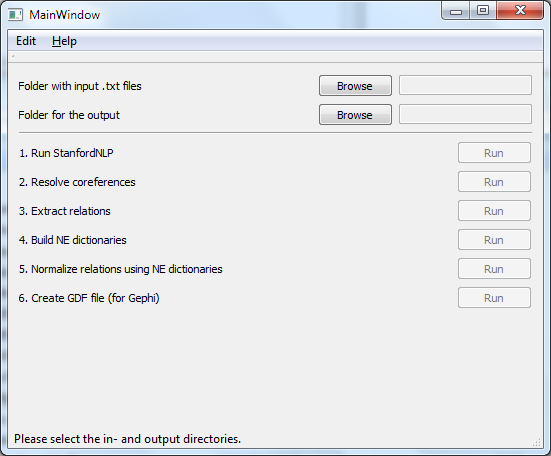
\includegraphics[width=0.8\textwidth]{images/Application}
    \caption{The application's main interface}
  \label{Application}
\end{figure}

The processing done by the application is fully automated and requires the user only to supply the input text files with the articles s/he wants to analyze. Then the processing is already structured in an optimal way, which eliminates the need to figure out what should be run and when. Note that the application requires the user to have Java, Perl and KNIME installed on the workstation. The paths to the binary files of those have to be specified in a ``Settings" window. In addition, relations may be extracted based on the mentioned confidence value, which is user-defined and may vary from 0 to 100\%.

Unfortunately, the progress bar was not integrated in the application to inform the user of the time left to wait. This is due to the time constraints. Also, the proper documentation is yet missing. Finally, currently the application is hardly customizable from the outside, therefore more settings should be added.

%
\section{Visualization}
%
Several modern tools were explored for the task of visualization. Among those, most notable are - GATE~\cite{gate}, KNIME~\cite{knime} and Gephi~\cite{gephi}. At first, on the stage of the coreference resolution, it was thought that GATE as a tool specifically designed for visual depiction of the text analysis results would suit best. However, it turned out that in terms of the visualization of the whole corpus processing results it is a very inflexible tool, which does not allow any user interaction with the visualization. It was decided, that GATE works best for the single document processing analysis in the situations when new or modified text mining algorithms are tested, but it does not fit the needs of a large scale mining.

After that, KNIME was used for basic visualizations almost on every processing stage. This tool is very helpful for the data input-output control purposes. Apart from that, KNIME was used for the most frequent keywords extraction and visualization in the form of an intuitive tag cloud (see Fig.~\ref{Cloud}) and for the keyword clustering and visualization, both k-means and hierarchical.
\begin{figure}[htbp]
  \centering
    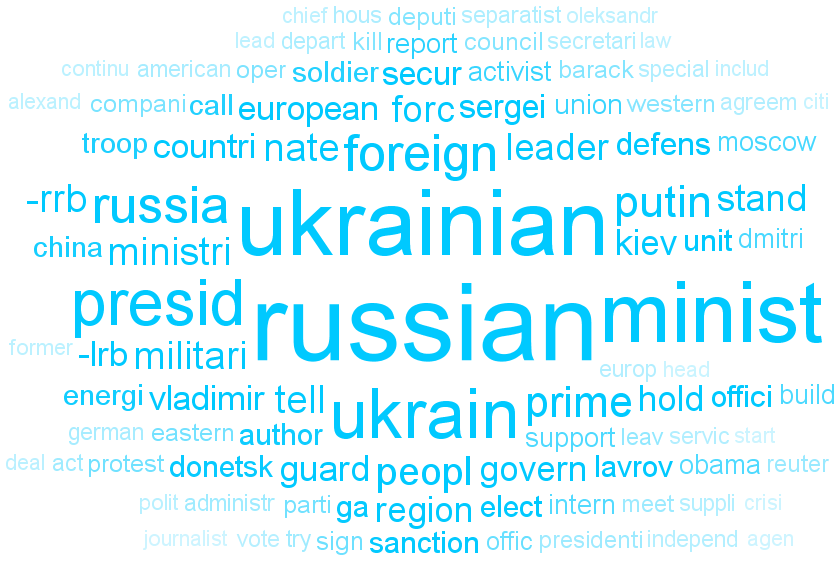
\includegraphics[width=0.8\textwidth]{images/Cloud}
    \caption{The most frequent stemmed keywords of the used corpus}
  \label{Cloud}
\end{figure}

The most efficient and meaningful visualizations of the extracted relations were produced by Gephi. Several types of representations were tried in it. It can be noticed that any of the representation tried suits well for the specific tasks. For example, relation types shown as nodes as well works good when the intention is to show the relation-centered graph (see Fig.~\ref{KievNetwork}), which is useful when specific relations are of the major interest (e.g. ``killed", ``accused", etc.). On the other hand, in the more general settings, when the task is more in the identification of what connects the entities together, a visualization where relations are just shown as edge labels works best (see Fig.~\ref{KievNetwork}).
\begin{figure}[htbp]
  \centering
    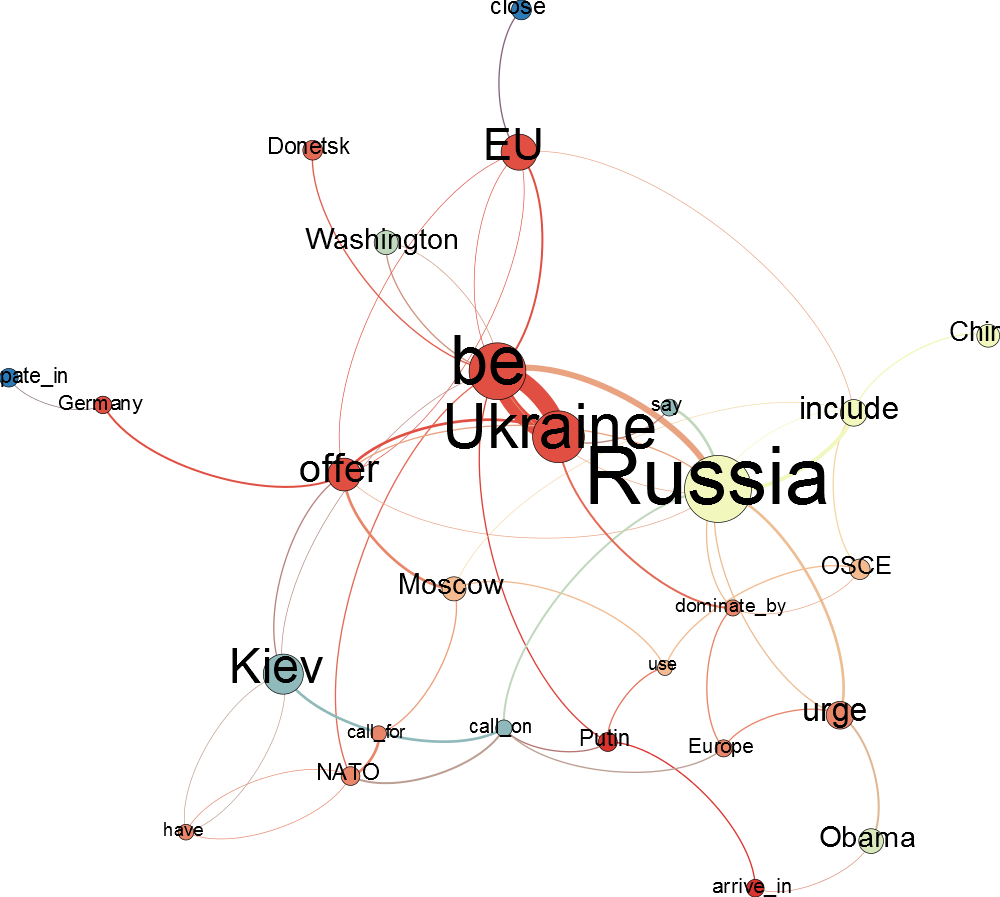
\includegraphics[width=0.8\textwidth]{images/AllRelations}
    \captionsetup{justification=centering}
    \caption{The most significant relations of the used corpus shown \\ as separate nodes (size - Betweenness Centrality, color - Modularity Class)}
  \label{AllRelations}
\end{figure}
\begin{figure}[htbp]
  \centering
    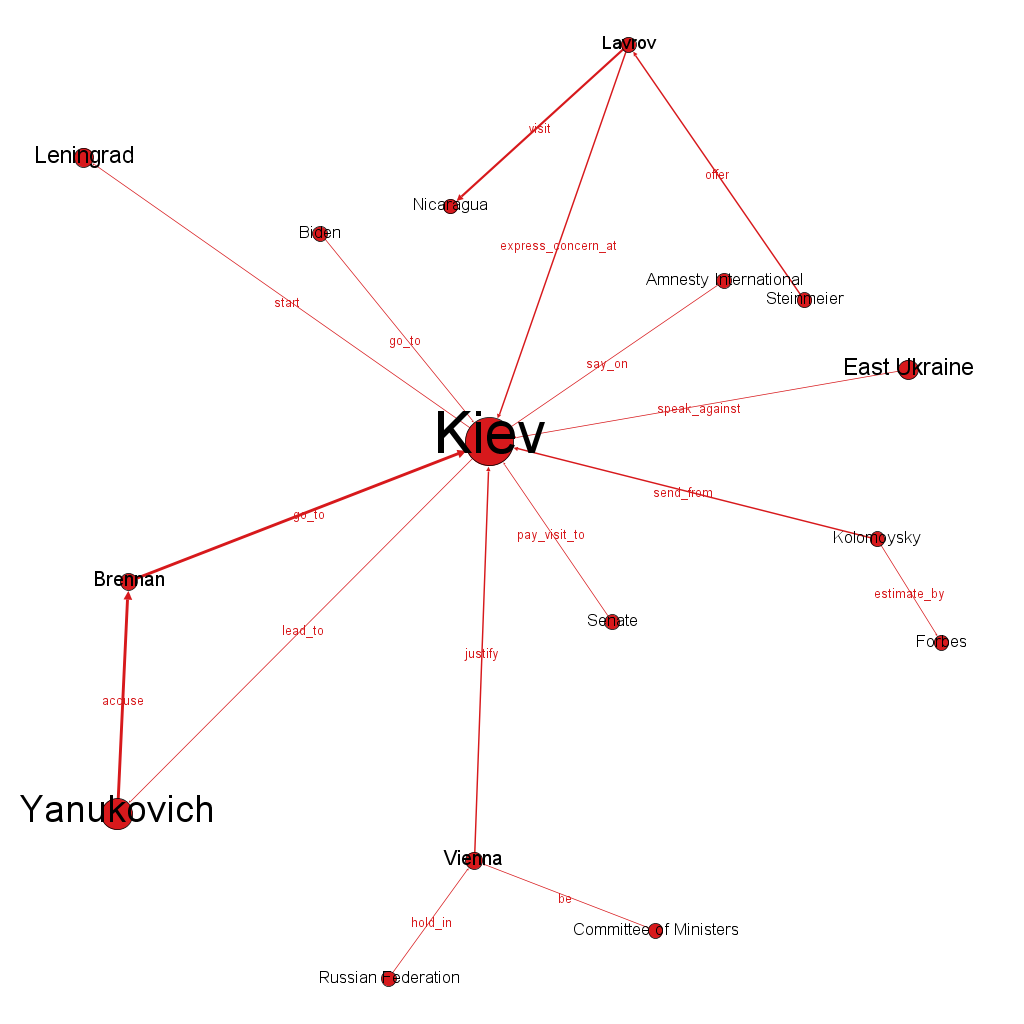
\includegraphics[width=0.8\textwidth]{images/KievNetwork}
    \captionsetup{justification=centering}
    \caption{Relational network of the entity ``Kiev", relations shown as labels (size - Eigenvector Centrality, color - Modularity Class)}
  \label{KievNetwork}
\end{figure}
% 
\section{Discussion}
%
As can be seen from the Visualizations, the most occurring relations within the corpus dominate the graph of all the relations. Furthermore, since strong words and verbs that probably represent opinions and subjective facts are not used very often, they are filtered out and are not presented in the graph. This leaves only the most occurring relations and consequently the objective ones in the end. It must be noted that numeric facts, e.g. the number of casualties on a certain event and how it fluctuates over time, cannot be efficiently extracted. This happens due to the fact that many different events happen simultaneously and, since the data comes from many different agencies, there is enough noise to make extracting such events unfeasible. The graphical interface of the application provides a framework that makes it easy for the end user to provide the text files and get the extracted relations in a format that can be easily passed on visualization tools. 

Finally, some improvements that could raise the quality of the framework are the following. Firstly, in the relation extraction phase, negation handling  should improve the quality of the relations that are extracted. Furthermore, the algorithm of extracting entities from the relations can be improved. Every part of a sentence can have more than one entities within, but only the first is taken into account when matching the dictionary entities with the sentence. An approach that takes into account all the entities that appear in a part of a sentence could be implemented. This could create more combinations of relations, but it's not clear if it will improve the end result since it could introduce noise to the relations. Lastly, improving the interface that is provided with highly customizable parameters will make the application even less domain dependent.
%
\section{Conclusion and future work}
%
Extracting objective facts regarding the same events as published from different sources is not an trivial task. In this work, a framework that can accurately extract relations from a corpus of non-homogeneous text documents was presented. The results are given in a form of a graph and their analysis displays the power of the framework. Furthermore, a graphical user interface is provided that makes  the procedure of relation extraction easier the user. Finally, on the discussion section the advantages and drawbacks of the framework are presented as well as ideas about future work that will improve the quality and power of the currently implemented relation extraction techniques.
%
% ---- Bibliography ----
%
\begin{thebibliography}{99}
%

\bibitem {perl}
Holzner S (1999)
Perl core language little black book. 
Coriolis Group Books

\bibitem {reverb}
Fader A, Soderland S, Etzioni O (2011) 
Identifying relations for open information extraction. 
Proc. Conf. Empirical Methods in Nat. Lang. Proc. 1535--1545
Association for Computational Linguistics.

\bibitem {stanford}
De Marneffe MC, Manning CD (2008)
Stanford typed dependencies manual. \texttt{http://nlp.stanford.edu/software/dependencies\_manual.pdf}

\bibitem{gephi}
Bastian M, Heymann S, Jacomy M (2009)
Gephi: an open source software for exploring and manipulating networks.
ICWSM 361--362

\bibitem{knime}
Berthold MR, Cebron N, Dill F, Gabriel TR, Kötter T, Meinl T, Wiswedel B (2008)
KNIME: The Konstanz information miner.
Springer Berlin Heidelberg 319--326

\bibitem{gate}
Cunningham H, Maynard D, Bontcheva K (2011)
Text processing with gate.
Gateway Press CA.

\bibitem{bart}
Versley Y, Ponzetto SP, Poesio M, Eidelman V, Jern A, Smith J, Moschitti A (2008)
BART: A modular toolkit for coreference resolution.
Proc. 46th Annual Meeting of the Assoc Comp Ling on Human Lang Tech 9--12

\end{thebibliography}

\end{document}
